\documentclass{beamer}
\usepackage{luatexja}
\usepackage{newpxtext,newpxmath}
\usepackage{listings}
\usepackage{graphicx}
\usetheme{Luebeck}
\usecolortheme{seahorse}
\usefonttheme{structurebold,serif}
\setbeamertemplate{navigation symbols}{\usebeamerfont{footline}\insertframenumber/\inserttotalframenumber}

\title{ルービックキューブと群論}
\author{宇佐見 公輔}
\date{2020年10月3日}
\begin{document}
\maketitle

\begin{frame}
    \frametitle{自己紹介}

    職業:プログラマ / 趣味:数学

    \bigskip

    最近の活動(登壇・ブログ・Twitter):
    \begin{itemize}
        \item 平面の敷き詰めとルート系(2020年6月 / 日曜数学会)
        \item 四元数のはなし(2020年5月 / 関西日曜数学友の会)
        \item はじめて学ぶリー環 ノート(2020年4月〜 / Twitter)
        \item Ising 模型 ノート(2020年3月〜4月 / Twitter)
        \item Onsager 代数の話(2020年3月 / 京都某所)
        \item はじめて学ぶリー群 ノート(2020年1月〜3月 / Twitter)
    \end{itemize}
\end{frame}

\begin{frame}
    \frametitle{今日の話}

    今日はルービックキューブの話です。過去の発表内容とは特に関係ありません。

    \bigskip

    ルービックキューブを数学的に考えるにはどうするのかという話と、SageMath での計算の紹介になります。

    \begin{figure}
        
\includegraphics[scale=0.25]{images/logo_sagemath+icon_oldstyle.png}
    \end{figure}
\end{frame}

\begin{frame}
    \frametitle{ルービックキューブ}

    \begin{figure}
        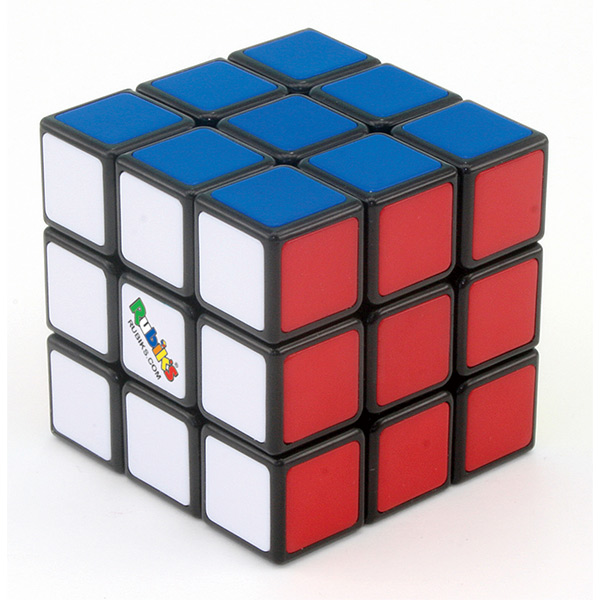
\includegraphics[scale=0.25]{images/rubik3.jpg}
        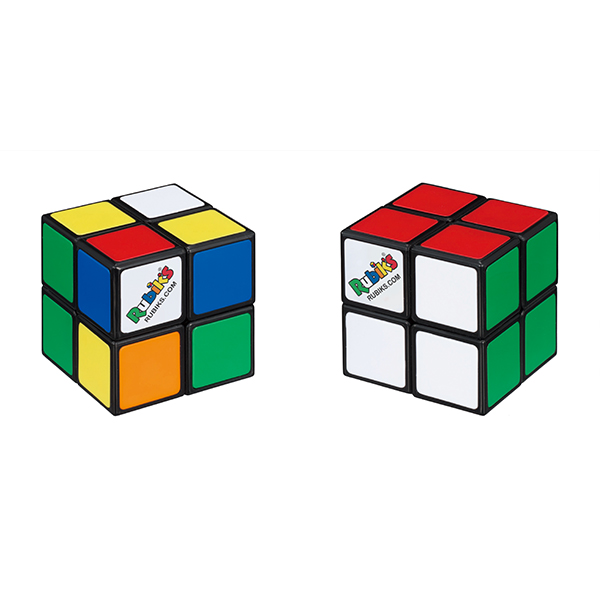
\includegraphics[scale=0.25]{images/rubik2.jpg}
    \end{figure}

    \(3 \times 3 \times 3\) が普通ですが、\(2 \times 2 \times 2\) など別サイズもあります。
\end{frame}

\begin{frame}
    \frametitle{ルービックキューブの数学的な解析}

    ルービックキューブに対する興味の持ち方は様々です。

    \begin{itemize}
        \item 6面完成させる解法は?
        \item スピードキューブ(完成までの時間を競う)
        \item キューブの機構はどうなっているのか?
    \end{itemize}

    \bigskip

    ここでは、ルービックキューブパズルを数学的に解析することを考えます。ルービックキューブは、群論の言葉を用いて記述することが可能です。
\end{frame}

\begin{frame}
    \frametitle{考察にあたっての前提}

    3次元空間の中でキューブの位置や向きを固定して考えます。キューブそのものを回転させることは考えません。

    キューブの操作は、各面を時計回りまたは反時計回りに90度ずつ動かすことを考えます。真ん中の列を回転させることはしません。

    \begin{figure}
        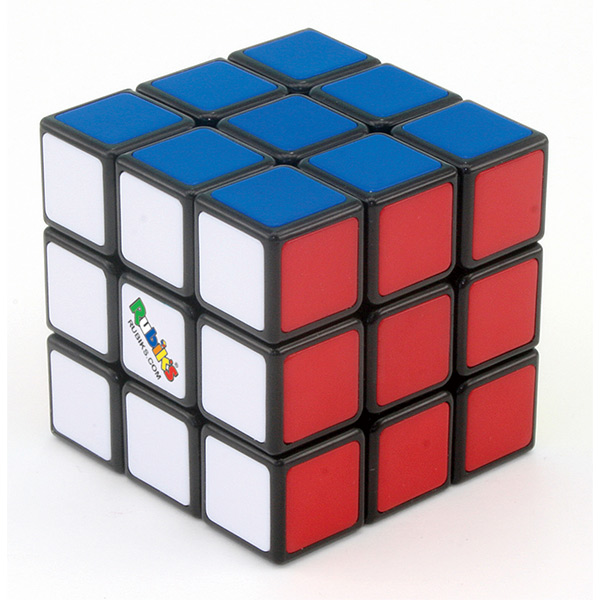
\includegraphics[scale=0.2]{images/rubik3.jpg}
    \end{figure}
\end{frame}

\begin{frame}
    \frametitle{小方体(cubelet)}

    \begin{itemize}
        \item 小方体:キューブを構成する小立方体。中心を除いて26個。
        \item 1面体:1つの面が外側に見えている小方体。6個。
        \item 2面体:2つの面が外側に見えている小方体。12個。
        \item 3面体:3つの面が外側に見えている小方体。8個。
    \end{itemize}

    \bigskip

    先ほどの前提から、1面体は動きません。2面体と3面体がキューブの操作によって移動します。
\end{frame}

\begin{frame}
    \frametitle{小面(facet)}

    キューブの各面を構成する正方形を小面と呼びます。各面で中央を除いて8個、全体で48個あります。

    \begin{figure}
        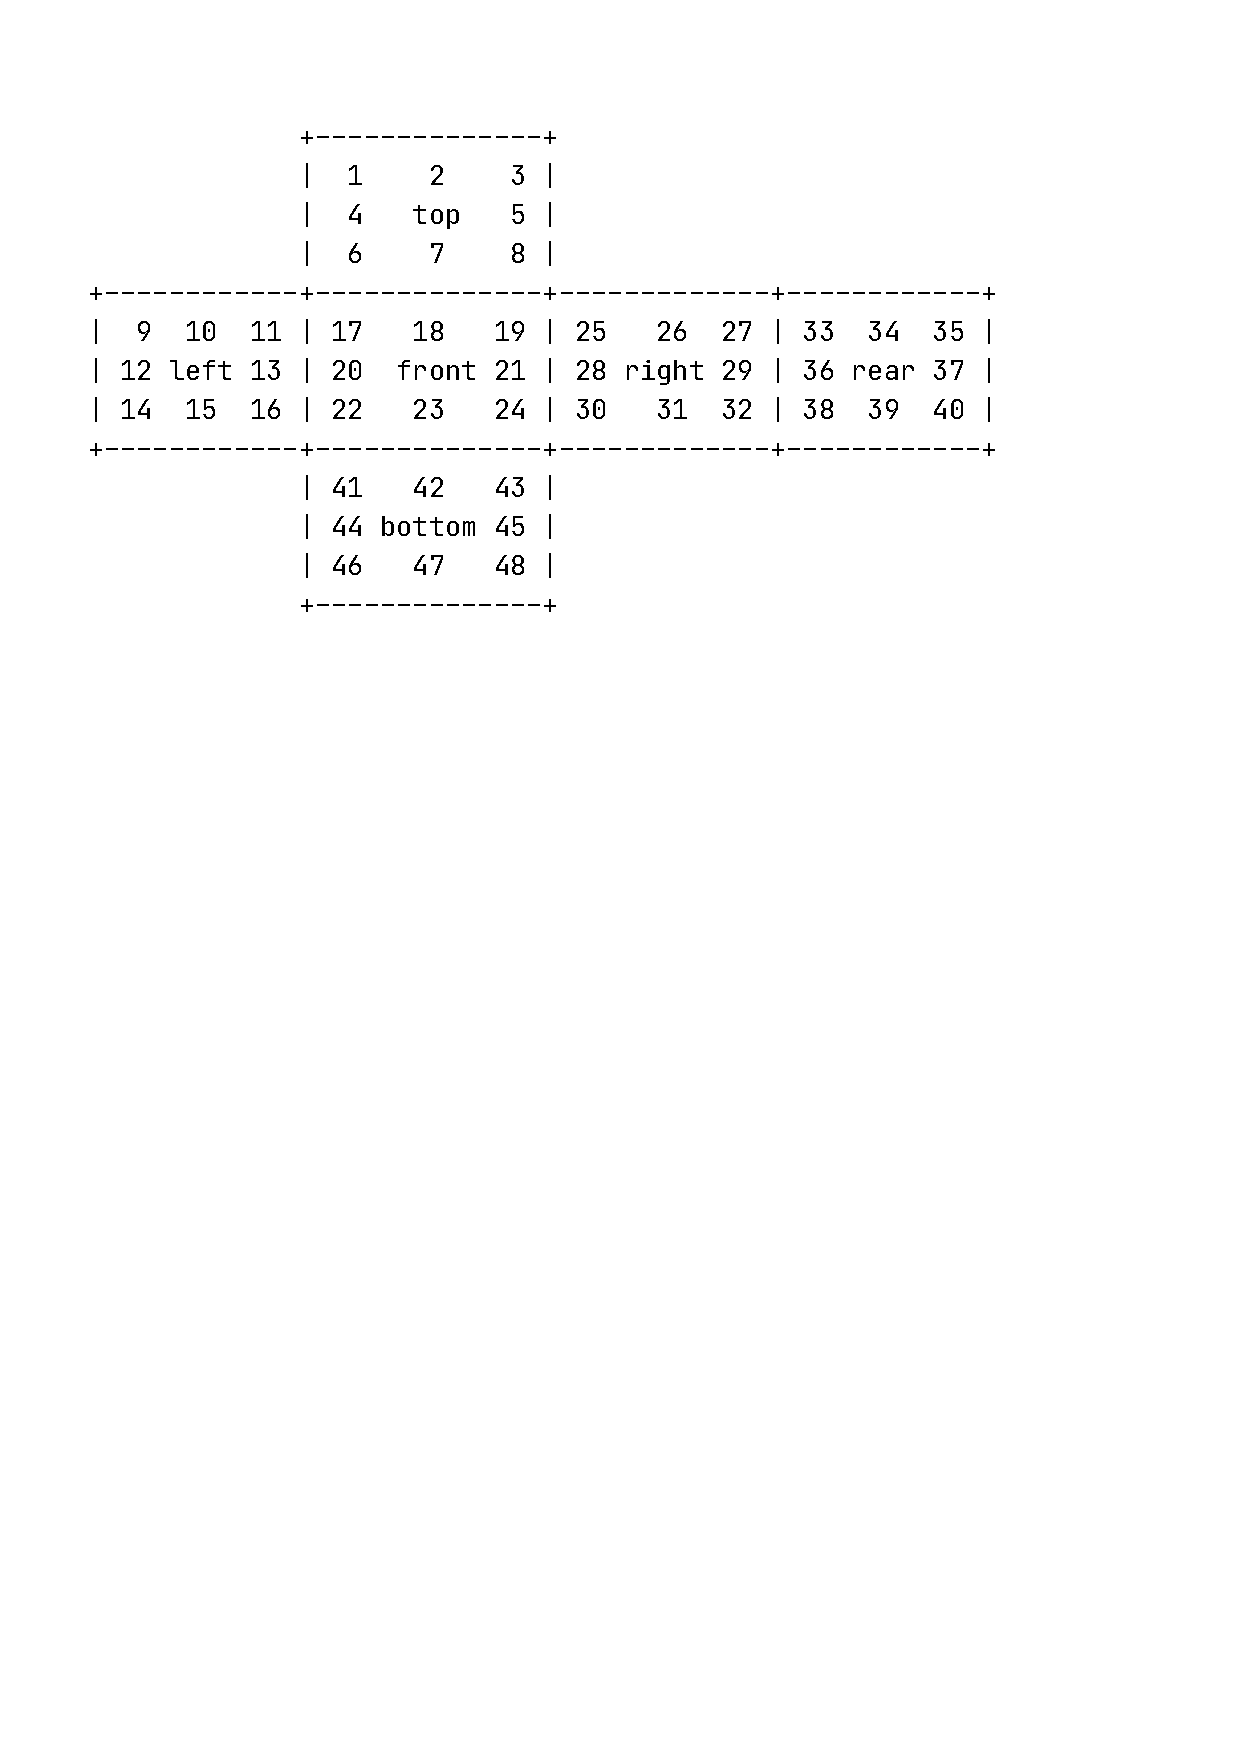
\includegraphics[scale=0.5]{images/display2d.pdf}
    \end{figure}

    番号づけの規則は何でもよいです。上図は SageMath の出力です。
\end{frame}

\begin{frame}
    \frametitle{小面のシングマスター記法}

    番号づけの代わりに、シングマスター記法という方法もあります。

    \begin{itemize}
        \item 上下左右前後の各面に \(u, d, l, r, f, b\) を割り当てる
        \item 2面体上の小面:xy 形式
              \begin{itemize}
                  \item x は小面を含む面
                  \item y は隣接する面
              \end{itemize}
        \item 3面体上の小面:xyz 形式
              \begin{itemize}
                  \item x は小面を含む面
                  \item y と z は隣接する面
              \end{itemize}
    \end{itemize}

    例:下図の 7 は \(uf\)、18 は \(fu\)、6 は \(ufl\)、17 は \(flu\) と書けます。

    \begin{figure}
        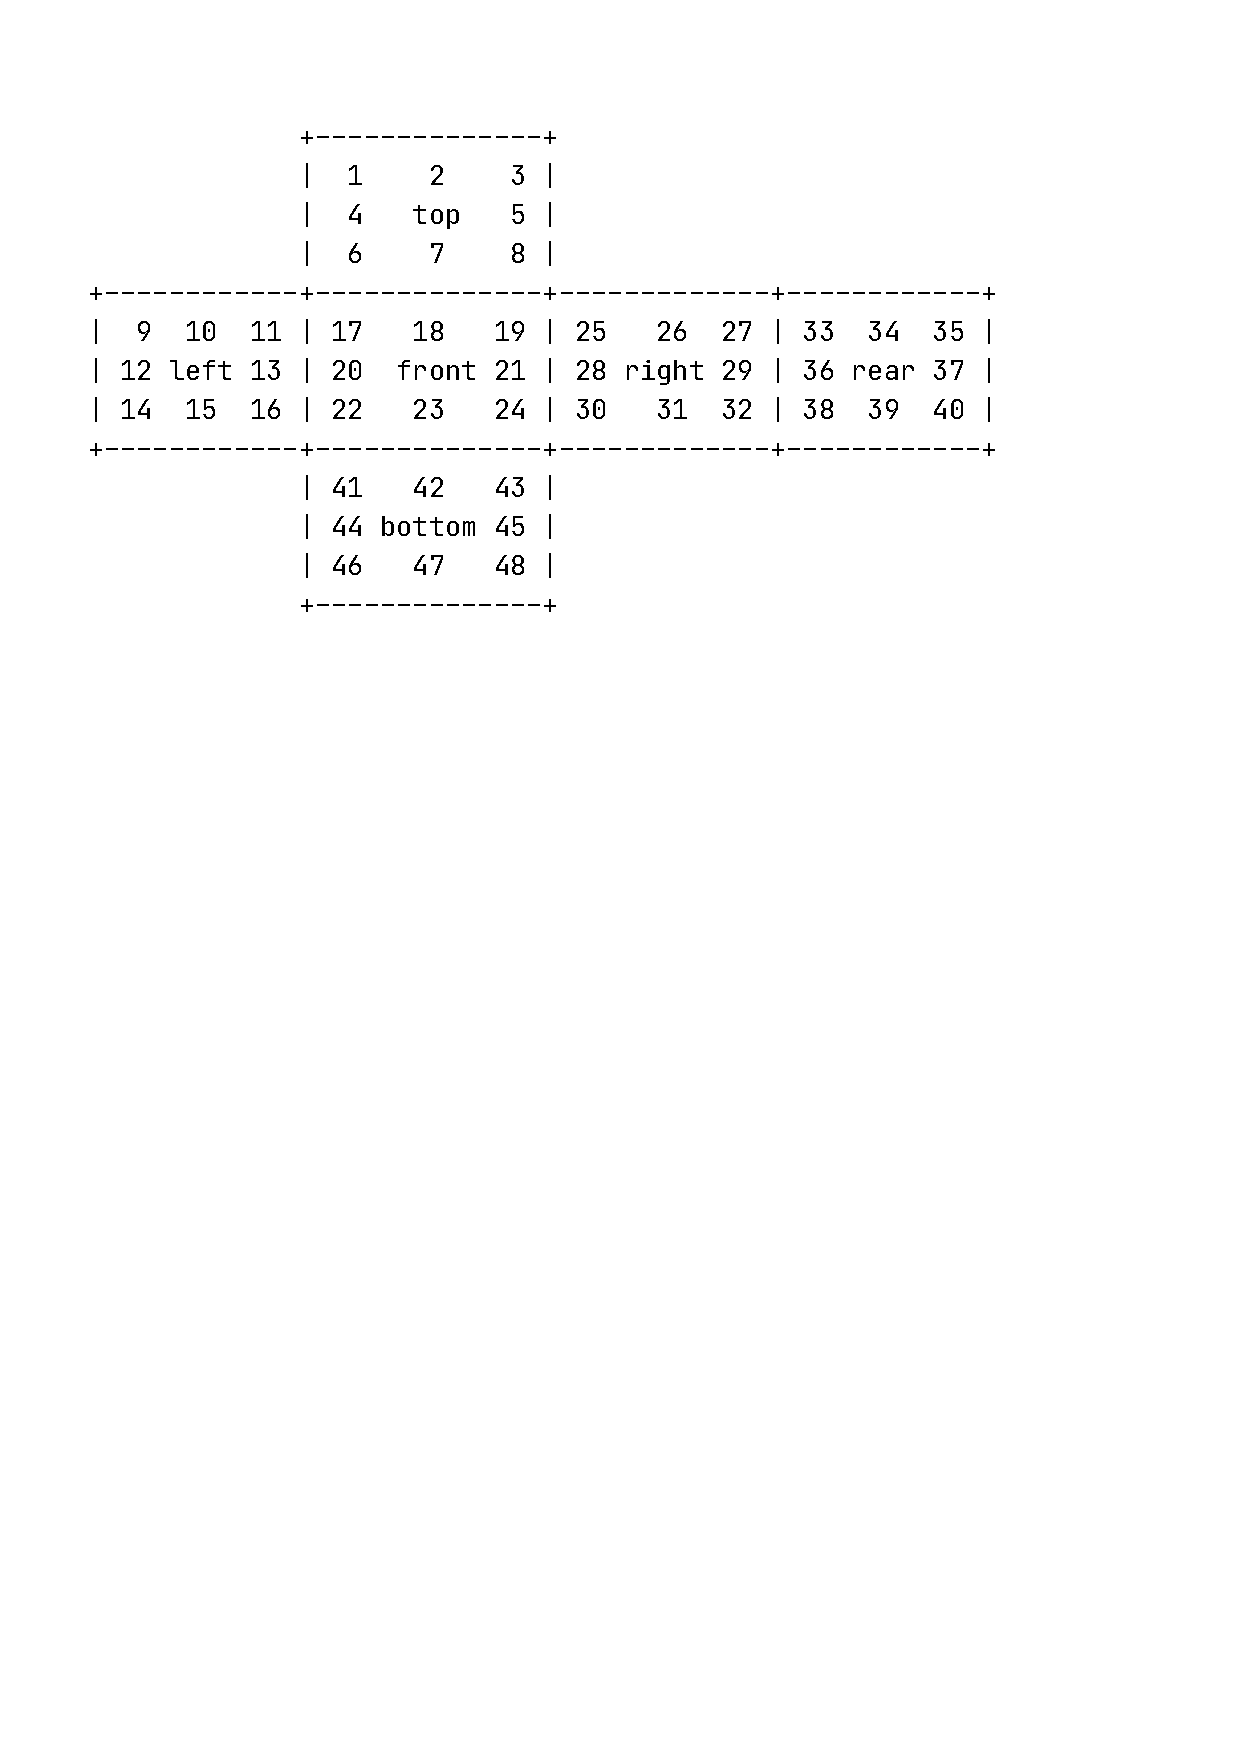
\includegraphics[scale=0.3]{images/display2d.pdf}
    \end{figure}
\end{frame}

\begin{frame}
    \frametitle{キューブ操作のシングマスター記法}

    \begin{figure}
        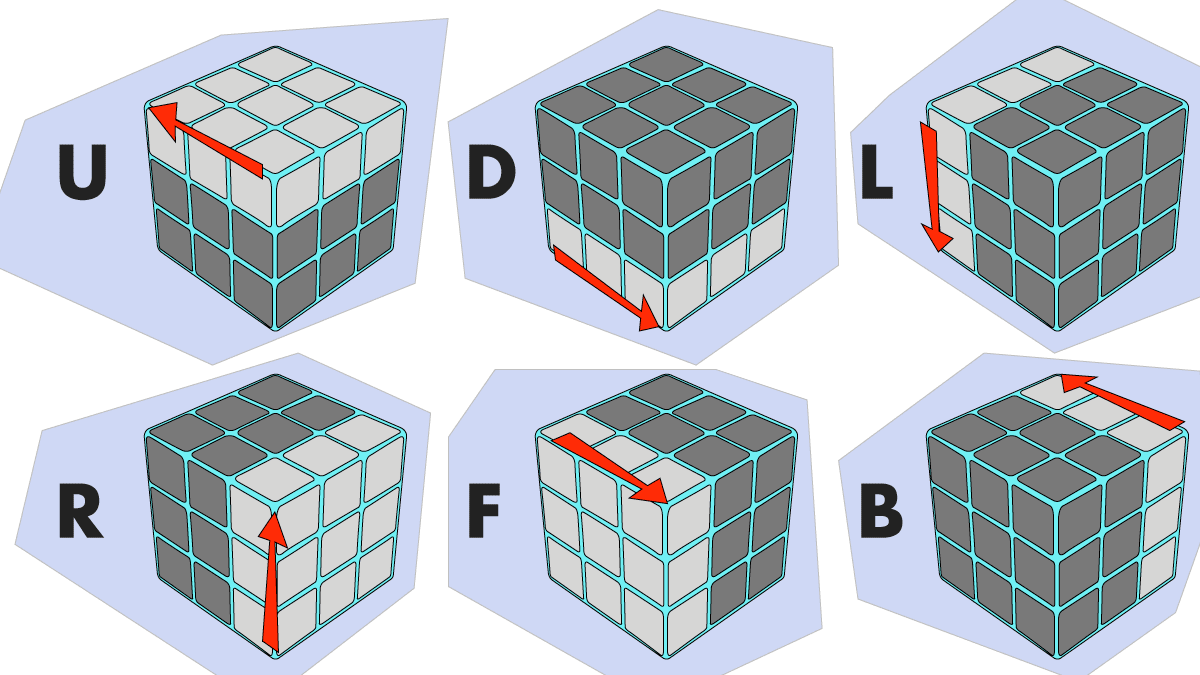
\includegraphics[scale=0.25]{images/singmaster.png}
    \end{figure}

    各面を時計回りに90度回転する操作を \(U, D, L, R, F, B\) と書くことにします。
\end{frame}

\begin{frame}
    \frametitle{キューブ操作と置換}

    \(X\) を小面48個の集合とします。キューブ操作は、\(X\) の置換写像であると考えることができます。

    \bigskip

    例えば操作 \(R\) は、以下のような置換です。小面を20個動かします。4個の元の巡回置換が5つ起こります。

    \begin{itemize}
        \item \(rf \mapsto ru \mapsto rb \mapsto rd \mapsto rf\)
        \item \(ruf \mapsto rub \mapsto rbd \mapsto rdf \mapsto ruf\)
        \item \(fr \mapsto ur \mapsto br \mapsto dr \mapsto fr\)
        \item \(fur \mapsto ubr \mapsto bdr \mapsto dfr \mapsto fur\)
        \item \(fdr \mapsto ufr \mapsto bur \mapsto dbr \mapsto fdr\)
    \end{itemize}
\end{frame}

\begin{frame}
    \frametitle{キューブ操作と置換 (2)}

    もうひとつ例を見ます。\(R\) を2回行った \(R^2\) は、以下のような置換です。2個の元の互換が10個起こります。

    \begin{itemize}
        \item \(rf \mapsto rb \mapsto rf\)
        \item \(ru \mapsto rd \mapsto ru\)
        \item \(ruf \mapsto rbd \mapsto ruf\)
        \item \(rub \mapsto rdf \mapsto rub\)
        \item \(fr \mapsto br \mapsto fr\)
        \item \(ur \mapsto dr \mapsto ur\)
        \item \(fur \mapsto bdr \mapsto fur\)
        \item \(ubr \mapsto dfr \mapsto ubr\)
        \item \(fdr \mapsto bur \mapsto fdr\)
        \item \(ufr \mapsto dbr \mapsto ufr\)
    \end{itemize}
\end{frame}

\begin{frame}
    \frametitle{対称群}

    集合 \(X\) の置換全体の集合 \(S_X\) は群になります。これを \(X\) の対称群と呼びます。

    \[
        S_X := \{f : X \to X \mid f \text{は全単射}\}
    \]

    キューブ操作(の組み合わせ)は、小面集合 \(X\) の対称群に含まれます。
\end{frame}

\begin{frame}
    \frametitle{ルービックキューブ群}

    小面集合 \(X\) の対称群 \(S_X\) の中にはキューブ操作の組み合わせだけでは実現できないものもあります。

    例えば、3面体のひとつをルービックキューブから取り外して、小面のうち2つの色を逆に貼り替えてからルービックキューブに戻す、ということをします。これは小面集合 \(X\) の置換にはなっていますが、キューブ操作だけでは元の配置に戻すことができません。

    \bigskip

    基本操作 \(U, D, L, R, F, B\) で生成される \(S_X\) の部分群 \(G\) を、ルービックキューブ群と呼びます。

    \[
        G := \langle U, D, L, R, F, B \rangle \subset S_X
    \]
\end{frame}

\begin{frame}
    \frametitle{SageMath}

    \begin{figure}
        
\includegraphics[scale=0.25]{images/logo_sagemath+icon_oldstyle.png}
    \end{figure}

    SageMath は数学関連のソフトウェアを統合したものです。SageMath には、ルービックキューブ群を扱うプログラムが最初から組み込まれています。
\end{frame}

\begin{frame}[fragile]
    \frametitle{ルービックキューブ群を SageMath で扱う}

    \begin{lstlisting}[language=Python]
sage: rubik = CubeGroup()
sage: rubik.plot_cube("")
sage: rubik.plot3d_cube("")
    \end{lstlisting}

    \begin{figure}
        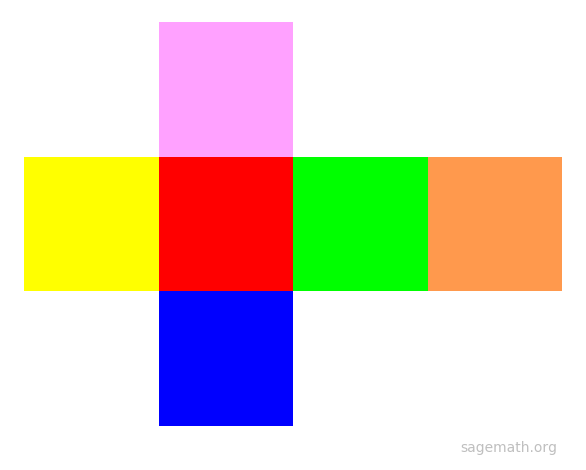
\includegraphics[scale=0.35]{images/plot_cube.png}
        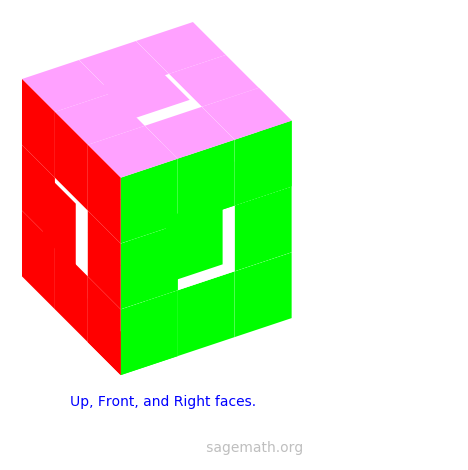
\includegraphics[scale=0.35]{images/plot3d_cube.png}
    \end{figure}
\end{frame}

\begin{frame}[fragile]
    \frametitle{ルービックキューブ群を SageMath で扱う (2)}

    \begin{lstlisting}[language=Python]
sage: rubik = CubeGroup()
sage: rubik.plot_cube("R")
sage: rubik.plot_cube("R*U")
    \end{lstlisting}

    \begin{figure}
        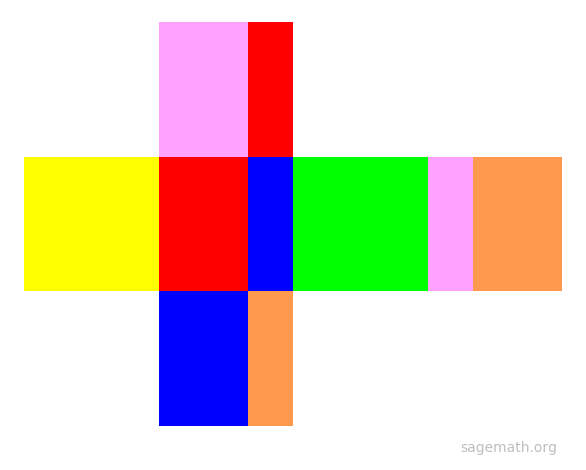
\includegraphics[scale=0.35]{images/plot_cube_R.png}
        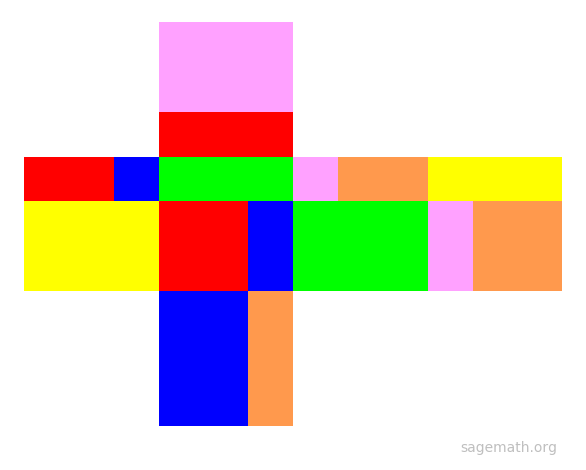
\includegraphics[scale=0.35]{images/plot_cube_RU.png}
    \end{figure}
\end{frame}

\begin{frame}[fragile]
    \frametitle{SageMath とシングマスター記法}

    \begin{lstlisting}[language=Python]
sage: rubik = CubeGroup()
sage: rubik.display2d("")
    \end{lstlisting}

    \begin{figure}
        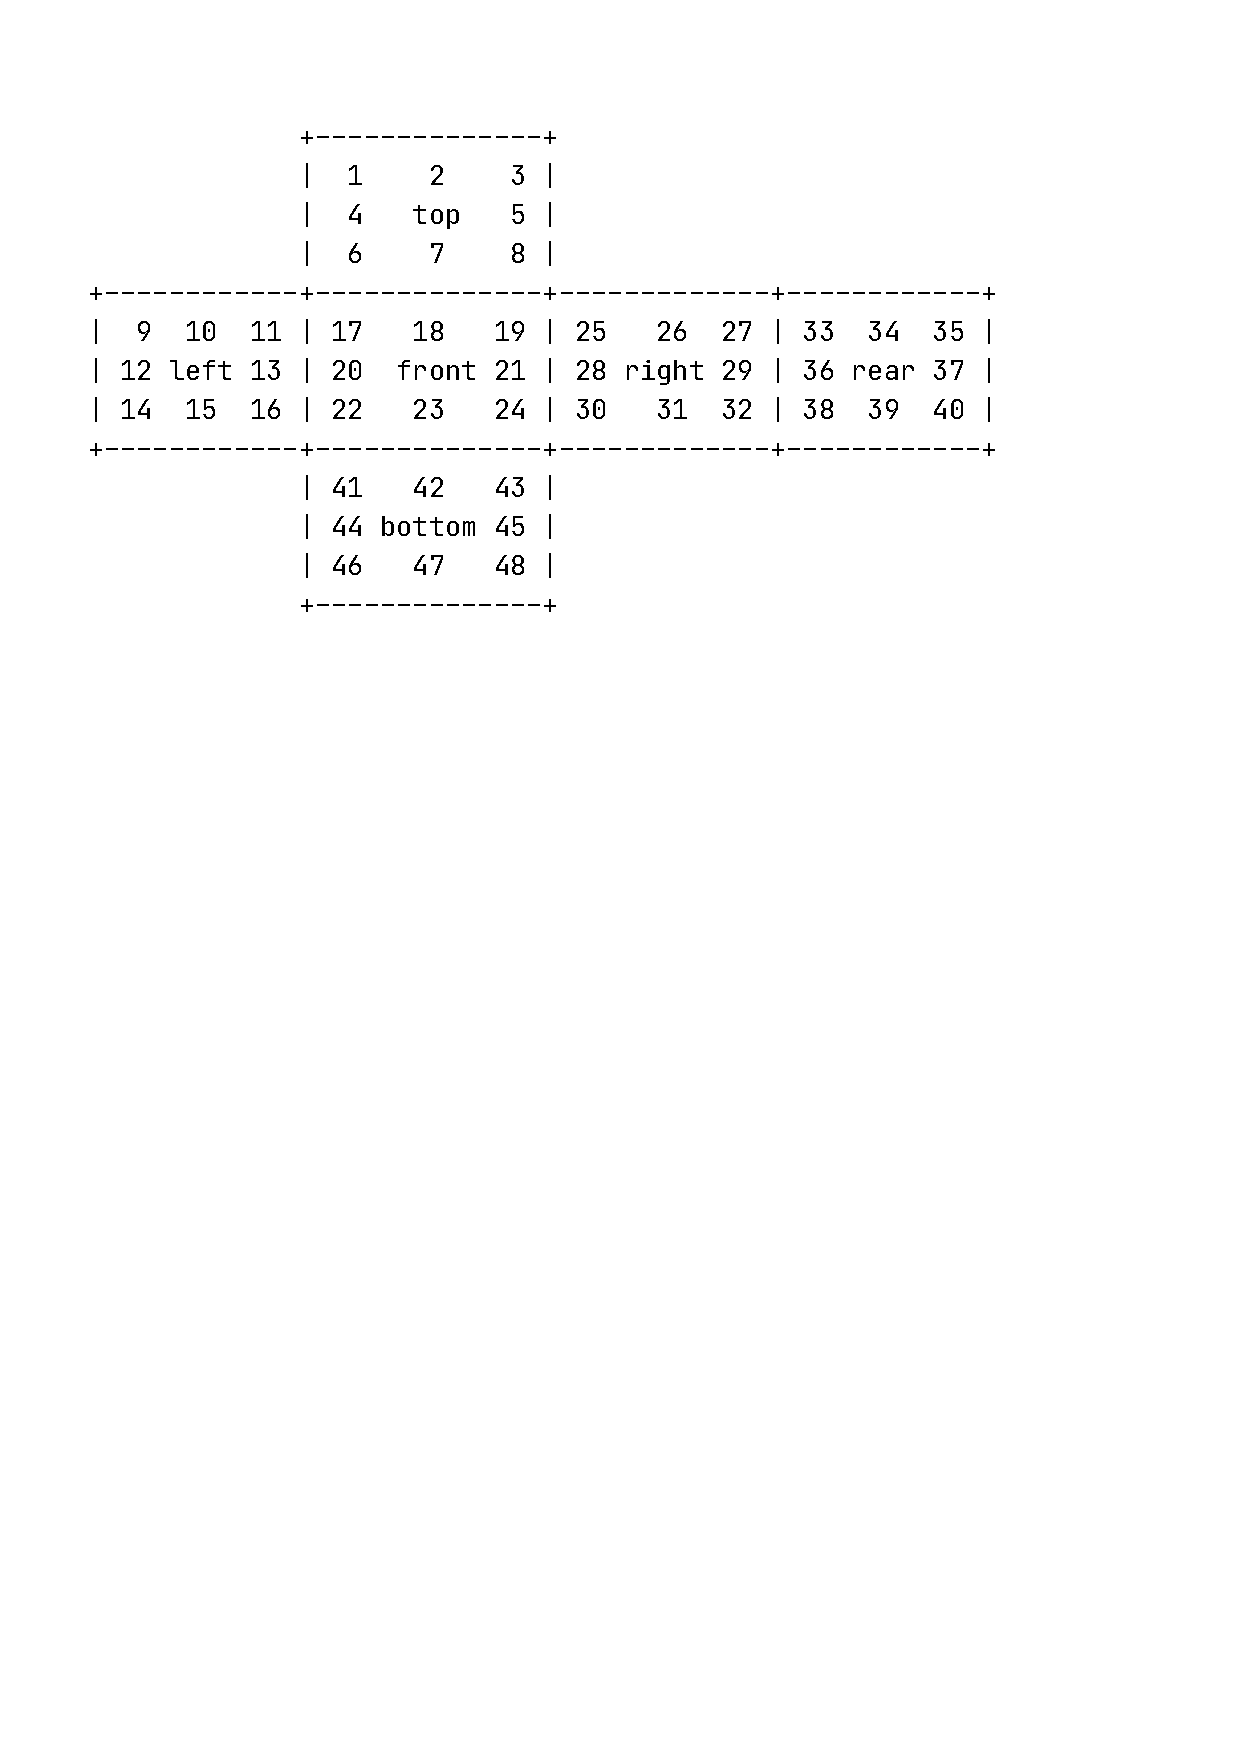
\includegraphics[scale=0.3]{images/display2d.pdf}
    \end{figure}

    \begin{lstlisting}[language=Python]
sage: from sage.groups.perm_gps.cubegroup import *
sage: index2singmaster(17)
'flu'
    \end{lstlisting}

\end{frame}

\begin{frame}[fragile]
    \frametitle{ルービックキューブ群の位数}

    ルービックキューブ群は定義から有限群ですが、その大きさがどれくらいなのか見てみます。

    \begin{lstlisting}[language=Python]
sage: rubik = CubeGroup()
sage: rubik.order()
43252003274489856000
sage: rubik.order().factor()
2^27 * 3^14 * 5^3 * 7^2 * 11
    \end{lstlisting}
\end{frame}

\begin{frame}[fragile]
    \frametitle{元の位数}

    ルービックキューブ群の元の位数(\(g^m = 1\) を満たす最小の \(m\))も見てみましょう。

    \bigskip

    操作 \(R\) は4回行えば元に戻ります。

    \begin{lstlisting}[language=Python]
sage: R = rubik.move("R")[0]
sage: R.order()
4
    \end{lstlisting}

    ルービックキューブ群には位数 \(1260\) の元があります。そのひとつが \(R U^2 D^{-1} B D^{-1}\) です。これより大きい位数の元はありません。

    \begin{lstlisting}[language=Python]
sage: J = rubik.move("R*U^2*D^-1*B*D^-1")[0]
sage: J.order()
1260
    \end{lstlisting}
\end{frame}

\begin{frame}
    \frametitle{その他の豆知識}

    \begin{itemize}
        \item どんな配置でも20手以内で6面完成できることが知られています(ただし、180度回転も1手とみなして数えた場合。180度回転を2手とするときは26手となる)。
        \item ルービックキューブ群は単純群ではありません(非自明な正規部分群を持つ)。
        \item 分解の例:\(G \cong (\mathbb{Z}_{3}^{7} \times \mathbb{Z}_{2}^{11}) \rtimes ((A_{8} \times A_{12}) \rtimes \mathbb{Z}_{2})\)
    \end{itemize}
\end{frame}

\begin{frame}
    \frametitle{まとめ・参考文献}

    ルービックキューブ群は群論の題材として(ちょっと大きいですが)良いものだと思います。また、SageMath を使うといろいろ遊べるのも良いと思います。

    \bigskip

    参考文献:

    \begin{itemize}
        \item David Joyner、群論の味わい −置換群で解き明かすルービックキューブと15パズル−
        \item 島内剛一、ルービック・キューブと数学パズル
    \end{itemize}
\end{frame}

\end{document}
